Die Entwicklung von Zusatzmodulen und Erweiterungen ist angesichts des modularen 
Aufbaukonzepts der Sage Office Line möglich. Die Einbindung von Erweiterungen wird 
mit einer eigenentwickelten Methode von Sage, namens DCM realisiert. Die Abkürzung
DCM steht für Dynamic Link Library\footnote{\label{foot:dll}Dynamic Link Library: 
Dynamische Programmbibliothek für Microsoft Betriebssysteme. (DLL) \cite{dll}} 
Common Method. Mit dieser Methode können Anpassung an der Sage Office Line auf Basis
des Microsoft .NET Frameworks\footnote{\label{foot:framework}Framework: Grundstruktur 
/ Rahmenwerk zur Bestimmung der Software-Architektur. Es besteht aus mehreren Klassen, 
die zusammenarbeiten und wieder verwendbare Entwürfe darstellen. \cite{framework}} 
vorgenommen werden. Mit Hilfe von DCM werden die Anpassungen mit der verwendeten 
Technologie der Sage Office Line auf Basis von Microsoft Access in Verbindung mit dem
Microsoft Component Object Model Frameworks (COM) verbunden.

\subsection{Projektstruktur}
Im ersten Schritt begann ich mit der Konstruktion der in Abbildung \ref{fig:paketdiagrammghs}
zu sehenden Projektstruktur. Zur Orientierung diente der vorher aufgestellte Umsetzungsplan.

\begin{figure}[H]
    \centering
    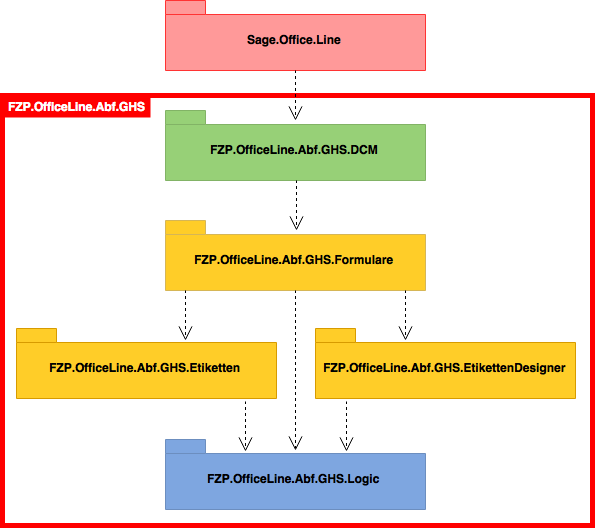
\includegraphics[height=240pt, width=300pt]{paketdiagramm_ghs_3.png}
    \caption[Paketdiagramm FZP.OfficeLine.Abf.GHS]
    {\small{Paketdiagramm FZP.OfficeLine.Abf.GHS}}
    \label{fig:paketdiagrammghs}
\end{figure}

\noindent
Das Projekt \emph{FZP.OfficeLine.Abf.GHS} unterteilt sich in 3 Bereiche. Das grün gefärbte
Paket stellt die Schnittstelle zwischen der Sage Office Line und dem Etikettendruckmodul 
dar. 

\begin{figure}[H]
    \centering
    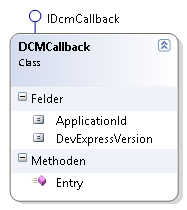
\includegraphics[height=100pt, width=90pt]{FZP_OfficeLine_Abf_GHS_DCM.png}
    \caption[Klassendiagramm FZP.OfficeLine.Abf.GHS.DCM]
    {\small{Klassendiagramm FZP.OfficeLine.Abf.GHS.DCM}}
    \label{fig:kddcm}
\end{figure}

\noindent
Die Schnittstelle, welche in Abbildung \ref{fig:kddcm} zu sehen ist, benötigt eine Klasse, 
welche das \emph{IDcmCallback} Interface von Sage implementiert. Dieses Interface stellt eine 
Methode namens \emph{Entry} zur Verfügung, welche ausimplementiert werden muss. Über diese 
Methode erhält man ein Kontext - Objekt, welches mit unterschiedlichen Daten (Kundennummer, 
Artikelnummer, Belegdaten, etc.) aus der Sage Office Line befüllt und in der Schnittstelle 
ausgelesen werden kann. 

\noindent
Die in der Abbildung \ref{fig:paketdiagrammghs} dargestellten gelb 
gefärbten Pakete repräsentiert die graphische Oberfläche des Moduls. Das Paket 
\emph{FZP.OfficeLine.Abf.GHS.Formulare} enthält die Klassen zur Erzeugung der Formulare. Die 
Formulare dienen einerseits zur Auswahl der Anzahl der zu druckenden Etiketten und deren 
Größe (\emph{frmGhsAuswahlEtiketten}). Auf der anderen Seite steht die Erfassung der Merkmale 
nach \emph{GHS/CLP} Verordnung für die einzelnen Artikel (\emph{frmGhsMerkmalErfassungsmaske}). 

\begin{figure}[H]
    \centering
    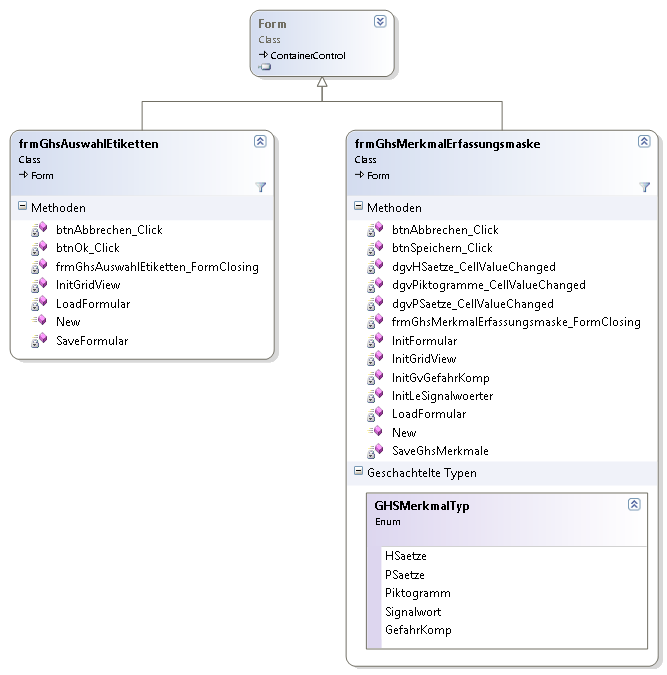
\includegraphics[height=290pt, width=290pt]{FZP_OfficeLine_Abf_GHS_Formulare_2.png}
    \caption[Klassendiagramm FZP.OfficeLine.Abf.GHS.Formulare]
    {\small{Klassendiagramm FZP.OfficeLine.Abf.GHS.Formulare}}
    \label{fig:kdformulare}
\end{figure}

\noindent
Das nächste Bestandteil ist das Paket \emph{FZP.OfficeLine.Abf.GHS.Etiketten}, welche die
notwendigen Klassen für die Erstellung der fest definierten Etiketten enthält. Für die
Etikettenerstellung kommt neben dem \emph{.NET} Framework, ein Framework der Firma 
Developer Express Inc. (DevExpress) zum Einsatz, welches die \emph{.NET} Winforms Steuerelemente 
im Funktionsumfang erweitert und zusätzlich die Handhabung erleichtert \cite{devexpress}. Zum Einen
enthält das Paket die Klasse \emph{GHSEtikettenAuswahl}, welche die Erstellung der Etiketten
anhand der übergebenen Füllmenge erzeugt, obendrein beinhaltet das Paket die konkreten Klassen 
für die einzelnen Etikettentypen. Außerdem sind die Gefahrenpiktogramme als Resourcen Dateien hinterlegt. 

\begin{figure}[H]
    \centering
    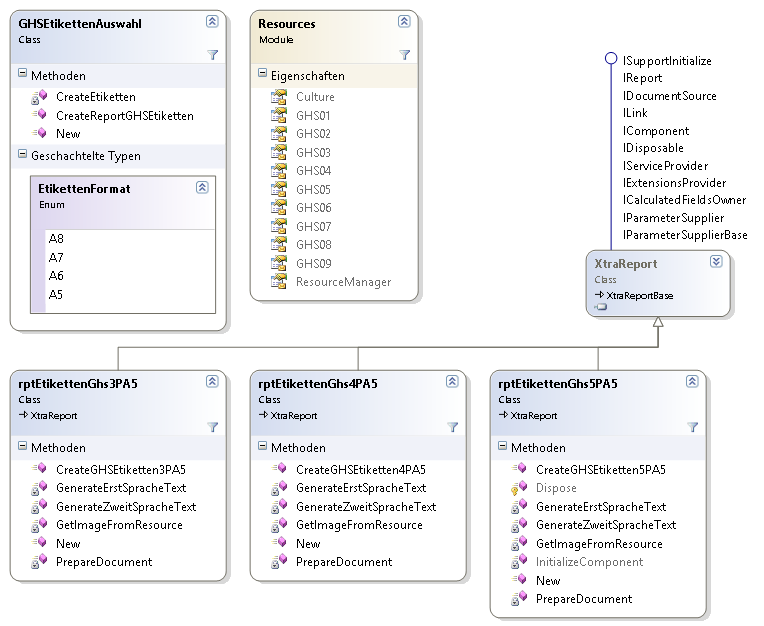
\includegraphics[height=300pt, width=\textwidth]{FZP_OfficeLine_Abf_GHS_Etiketten_2.png}
    \caption[Klassendiagramm Auszug FZP.OfficeLine.Abf.GHS.Etiketten]
    {\small{Klassendiagramm Auszug FZP.OfficeLine.Abf.GHS.Etiketten}}
    \label{fig:kdetiketten}
\end{figure}

\noindent
Die dritte Komponente ist das Paket \emph{FZP.OfficeLine.Abf.GHS.EtikettenDesigner}, 
welche die notwendigen Klassen für die Erstellung von selbst definierten Etiketten 
enthält. Auch hier wird neben dem \emph{.NET} Framework, dass Framework von \emph{DevExpress} 
verwendet. Leider wurde aufgrund zeitlicher und finanzieller Gründe der Etikettendesigner 
abschließend nicht von unserem Kunden beauftragt und ist somit nicht über die Planungsphase 
hinaus gekommen. Aus diesem Grund liegt nur eine grobe Klassenstruktur vor (siehe Abbildung 
\ref{fig:kdetikettendesigner}). 

\begin{figure}[H]
    \centering
    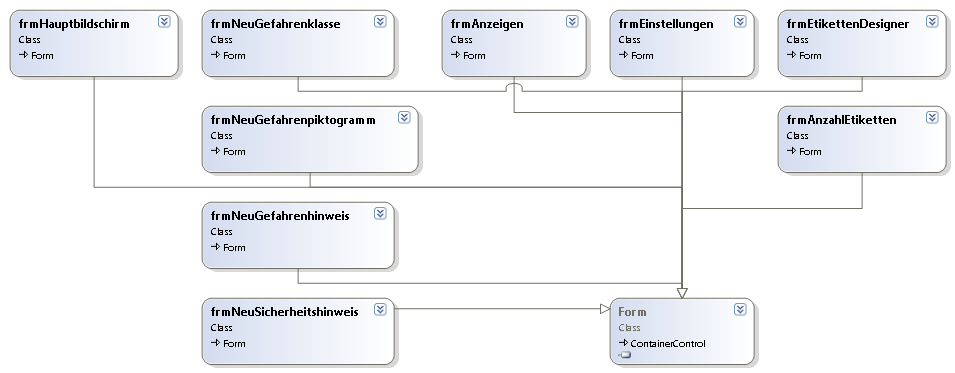
\includegraphics[height=250pt, 
    width=\textwidth]{FZP_OfficeLine_Abf_GHS_EtikettenDesigner_2.png}
    \caption[Klassendiagramm FZP.OfficeLine.Abf.GHS.EtikettenDesigner]
    {\small{Klassendiagramm FZP.OfficeLine.Abf.GHS.EtikettenDesigner}}
    \label{fig:kdetikettendesigner}
\end{figure}

\noindent
Das letzte Element des Moduls ist das blau gefärbte Paket \emph{FZP.OfficeLine.Abf.GHS.Logic}.
In diesem Paket befindet sich die Businesslogik des gesamten Etikettendruckmoduls. Das 
Hauptziel des Pakets ist die strikte Trennung der graphischen Oberfläche von der 
Businesslogik. Durch diese Trennung ist es möglich die graphische Oberfläche auszuwechseln ohne 
die Buisnesslogik ändern zu müssen. Das Paket beinhaltet Klassen zur Datenhaltung und Manipulation 
der Merkmale nach \emph{GHS/CLP} Verordnung. Die Klassen erben von der \emph{KeyedCollection} - Klasse, 
welche "'eine Basisklasse für eine Auflistung bereitstellt"' und mit Schlüssel - Wert Paaren 
arbeitet \cite{coll}. Die Speicherung der Daten erfolgt in der MS SQL Datenbank der Sage 
Office Line. Des Weiteren stellt das Paket zur Regelung der Datenbankverbindung und Ausführung 
von SQL - Abfragen Hilfsklassen zur Verfügung (GHSMerkmal, GHSMerkmalErweiterung, MandantHelper). 
Daneben steht eine Klasse zur Größenänderung von Bildern, Umwandlung von Bilder in den Datentyp 
\emph{Byte Arrays} und umgekehrt zur Verfügung (ImageHelper). Weiterhin existiert eine Klasse zur
Aufbereitung der Daten aus der Datenbank zur Verwendung in der graphischen Oberfläche (GHSMerkmalHelper) 
(siehe Abbildung \ref{fig:kdlogik}).

\begin{figure}[H]
    \centering
    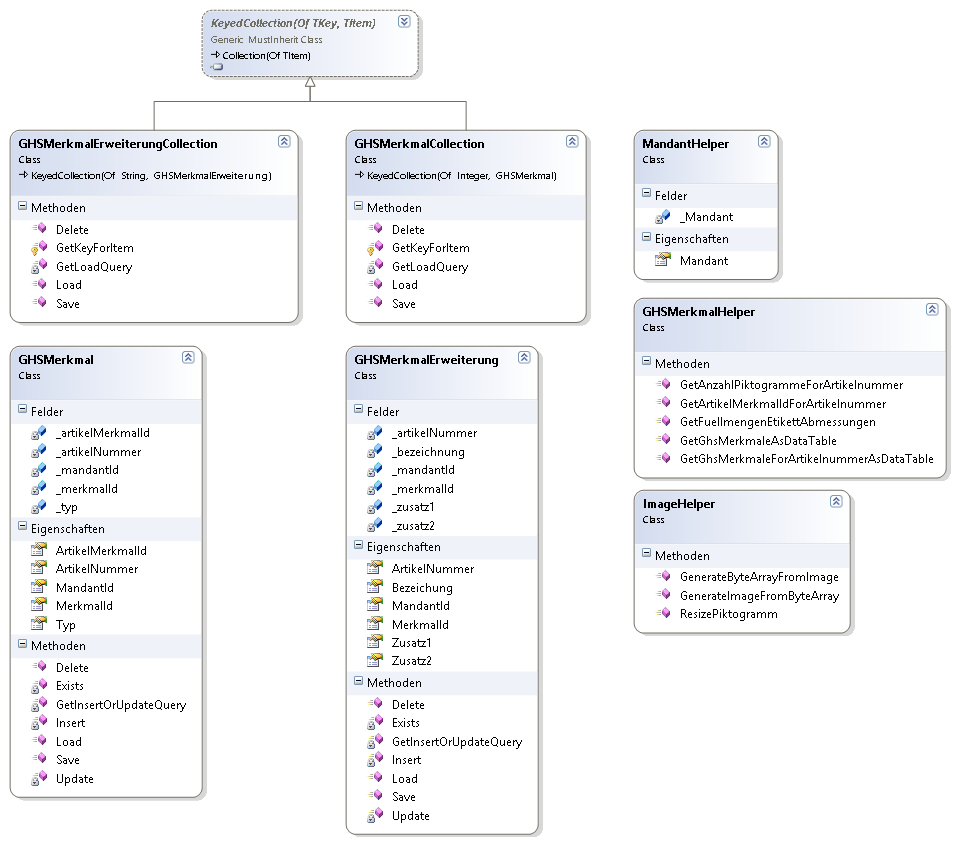
\includegraphics[height=450pt, width=\textwidth]{FZP_OfficeLine_Abf_GHS_Logic_2.png}
    \caption[Klassendiagramm FZP.OfficeLine.Abf.GHS.Logic]
    {\small{Klassendiagramm FZP.OfficeLine.Abf.GHS.Logic}}
    \label{fig:kdlogik}
\end{figure}

\subsection{Funktionsweise}

Im nachfolgenden Abschnitt ist die Funktionsweise des Moduls anhand von Quellcodeauszügen
erklärt. Das Etikettendruckmodul wird, wie in Abschnitt \ref{subsubsec:erweiterungartikelstamm}
bereits erläutert wurde, an mehreren Stellen aufgerufen. Dabei kann der Anwender
in der Sage Office Line den Menüpunkt "'GHS Merkmale"' in den Artikelstammdaten auswählen
(Case Zweig 201). Nach der Speicherung von Verkaufsbelegen wird das Ereignis 
"'FZPGHSDruckauftrag"' ausgelöst (Case Zweig 200). Das Modul arbeitet den folgenden Quellcode ab:
\newline
\newline
\newline
\begin{lstlisting}[style=A, caption=Aufruf Formulare aus Sage Office Line (COM),
label={code:addin}]
    Select Case nMode
        '# Aufruf Formular Druckauftrag
        Case 200
            Set oBagDCM = New ParameterBag
            Set oBagDCM.oItem("Beleg") = goStack.oBag.oItem("Beleg")
            Call goMandant.bExecuteDCMCustomizing("FZPGHSDruckauftrag", oBagDCM)
            
        '# Aufruf Formular Erfassung GHS Merkmale
        Case 201
            Set oBagDCM = New ParameterBag
            oBagDCM.sItem("Artikelnummer") = gsParameter(sArgs, "Artikelnummer", "")
            Call goMandant.bExecuteDCMCustomizing( _
            "FZPGhsErfassungMerkmaleArtikelstamm", oBagDCM)
    End Select
\end{lstlisting}

\noindent
Wie zu sehen ist wird in beiden Case Zweigen ein Objekt von Typ \emph{ParameterBag} erzeugt. 
Dieses Objekt dient zur Übergabe und Haltung von Daten aus der Sage Office Line in unser 
Modul. Der Einstiegspunkt in das Etikettendruckmodul ist zu sehen in der Zeile 6 und 
Zeile 12 des Quellcodes. Die Methode \emph{bExecuteDCMCustomizing} benötigt 2 Parameter. 
Der erste Parameter muss eine eindeutige Zeichenketten sein, welche zur Identifikation in
unserem Modul genutzt wird, um festzustellen welche Funktion ausgewählt wurde (siehe Listing
\ref{code:addin}: Zeile 6 und 12 und Listing \ref{code:dcmcallback}: Zeile 2 und 10). Als 
zweiter Parameter wird das erzeugte \emph{ParameterBag} Objekt übergeben. Im 
Quellcodeauszug Nr. \ref{code:dcmcallback} sieht man die Auswertung der übergebenen
Zeichenkette in der \emph{Select Case Anweisung}, außerdem das Auslesen und die Verarbeitung des
Kontext - Objekts (siehe Zeile 4 - 6 und Zeile 12 - 14).

\begin{lstlisting}[style=A, caption=Verarbeitung Aufruf Formulare aus Sage Office Line (.NET),
label={code:dcmcallback}]
    Select Case context.Listname
        Case "FZPGHSDruckauftrag"
            '# Aufruf Formular zum Druck der Etiketten
            Dim dcmBeleg As Sagede.OfficeLine.Wawi.BelegEngine.DcmContextBeleg = _
            CType(context, Sagede.OfficeLine.Wawi.BelegEngine.DcmContextBeleg)
            Dim beleg As Sagede.OfficeLine.Wawi.BelegEngine.Beleg = dcmBeleg.Beleg
            Using druckAuftrag As New frmGhsAuswahlEtiketten(mandant, beleg)
                druckAuftrag.ShowDialog()
            End Using
        Case "FZPGhsErfassungMerkmaleArtikelstamm"
            '# Aufruf Formular zu Erfassung der GHS Merkmale
            Dim engine As DcmContextEngine = CType(context, DcmContextEngine)
            Dim artikelNummer As String = engine.ParameterBag.StringValues( _ 
            "Artikelnummer")
            Using merkmalErfassungsmaske As New frmGhsMerkmalErfassungsmaske(Mandant, _
            artikelNummer)
                merkmalErfassungsmaske.ShowDialog()
            End Using
    End Select
\end{lstlisting}

\noindent
Nach der Verarbeitung des Kontext-Objekts zur Verwendung der übergebenen Daten aus der Sage
Office Line folgt die Initialisierung der Formulare. Zum Einen für die Aufnahme der Merkmale nach 
\emph{GHS/CLP} Verordnung für den übergebenen Artikel (Abbildung \ref{fig:eperfassungsmaske})
oder zum Anderen für den Aufruf der Druckmaske (Abbildung \ref{fig:epdruckmaske}) (siehe Listing
\ref{code:dcmcallback} - Quellcodezeilen 7 - 9 plus 15 - 18).

\begin{figure}[H]
    \centering
    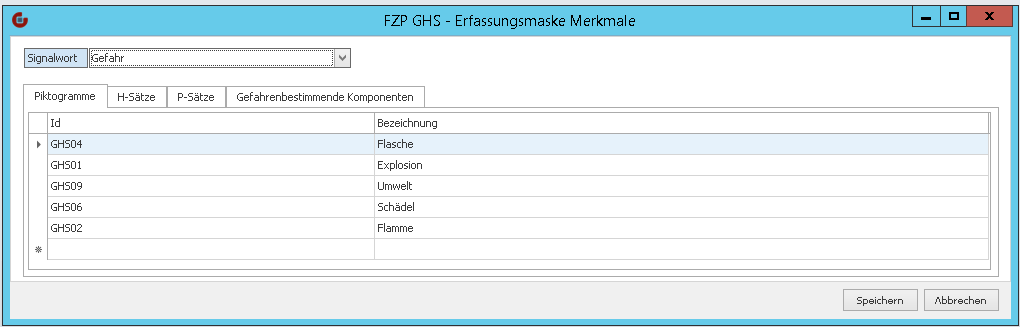
\includegraphics[height=160pt, width=\textwidth]{Erfassung_endprodukt_2.png}
    \caption[Endprodukt der Arikelstammdatenerfassung]
    {\small{Endprodukt der Arikelstammdatenerfassung}}
    \label{fig:eperfassungsmaske}
\end{figure}

\noindent
Die erste Möglichkeit ist die Erfassung der benötigten Merkmale nach \emph{GHS/CLP} Verordnung für 
jeden einzelnen Artikel (siehe Abbildung \ref{fig:eperfassungsmaske}). Durch Betätigung der Schaltfläche
zum Speichern werden die Informationen in die MS SQL Datenbank geschrieben (siehe Listing \ref{code:speichern}).
\newline
\begin{lstlisting}[style=A, caption=Auszug Speicherroutine GHS/CLP Merkmale (.NET),
label={code:speichern}]
    Public Class frmGhsMerkmalErfassungsmaske
        ...
        '# Aufruf Methode zur Speicherung GHS Merkmale im Formular 
        '# mittels Speichern Button
        '# ----------------------------------------------------------------
        '# Die eingegebenen Daten werden aus der GridView in eine DataTable 
        '# geschrieben. Anschlieszend werden alle Zeilen der DataTable 
        '# durchgegangen und die Daten in Objekte geschrieben und der 
        '# Collection hinzugefuegt und abschlieszend gespeichert.  
        Private Function SaveGhsMerkmale() As Boolean
            dgvHSaetze.UpdateCurrentRow()
            ...
            Dim hSaetze As DataTable = CType(dgcHSaetze.DataSource, DataTable)
            ...
            Dim ghsMerkmale As New GHSMerkmalCollection
            Dim ghsMerkmal As GHSMerkmal
            Dim artikelMerkmalId As Integer
            ...
            '# H-Saetze
            For Each row As DataRow In hSaetze.Rows
                ghsMerkmal = New GHSMerkmal
    
                If FZPCInt(row("ArtikelMerkmalId")) = 0 Then
                    artikelMerkmalId = _mandant.GetTan("FZPGHSArtikelMerkmal")
                Else
                    artikelMerkmalId = FZPCInt(row("ArtikelMerkmalId"))
                End If
                ghsMerkmal.ArtikelMerkmalId = artikelMerkmalId
                ghsMerkmal.MandantId = _mandant.Id
                ghsMerkmal.ArtikelNummer = _artikelNummer
                ghsMerkmal.Typ = GHSMerkmalTyp.HSaetze
                ghsMerkmal.MerkmalId = FZPCStr(row("MerkmalId"))
    
                ghsMerkmale.Add(ghsMerkmal)
            Next
            ...
            If ghsMerkmale.Save() Then
                Return True
            End If
        End Function
        ...
    End Class

    Public Class GHSMerkmalCollection
        Inherits System.Collections.ObjectModel.KeyedCollection(Of Integer, GHSMerkmal)
        ...
        '# Aufruf Speicheranweisung aller GHS Merkmal Objekte innerhalb der Collection
        Public Function Save() As Boolean
            For Each item As GHSMerkmal In Me
                item.Save()
            Next
        End Function
        ...
    End Class
    
    Public Class GHSMerkmal
        ...
        '# Ausfuehrung der Speicheranweisung fuer jedes GHS Merkmal
        '# ----------------------------------------------------------------
        '# Zuerst wird der SQL-Query mittels StringBuilder erstellt. Die @-Parameter 
        '# dienen als Platzhalter die durch die "sqlCommand.AppendInParameter()" 
        '# Anweisung durch die Daten aus dem GHS Merkmale Objekt ersetzt werden. 
        '# Mittels der Anweisung "sqlCommand.ExecuteNonQuery()" wird der SQL-Query 
        '# auf der Datenbank ausgefuehrt.
        Private Sub Save()
            Try
                Dim query As New System.Text.StringBuilder
                
                query.AppendLine("INSERT INTO FZPGHSArtikelMerkmal")
                query.AppendLine("(")
                query.AppendLine("  ArtikelMerkmalId,")
                query.AppendLine("  Mandant,")
                query.AppendLine("  Typ,")
                query.AppendLine("  MerkmalId,")
                query.AppendLine("  Artikelnummer")
                query.AppendLine(")")
                query.AppendLine("VALUES")
                query.AppendLine("(")
                query.AppendLine(" @ArtikelMerkmalId,")
                query.AppendLine(" @Mandant,")
                query.AppendLine(" @Typ,")
                query.AppendLine(" @MerkmalId,")
                query.AppendLine(" @Artikelnummer")
                query.AppendLine(")")
                
                Dim sqlCommand As IGenericCommand = 
                MandantHelper.Mandant.MainDevice.GenericConnection.CreateCommand( _
                GenericCommandType.SqlS
                tring, query.ToString, True)
                sqlCommand.AppendInParameter("ArtikelMerkmalId", GetType(Integer), _
                _artikelMerkmalId)
                sqlCommand.AppendInParameter("Mandant", GetType(Short), _mandantId)
                sqlCommand.AppendInParameter("Typ", GetType(Integer), _typ)
                sqlCommand.AppendInParameter("MerkmalId", GetType(String), _merkmalId)
                sqlCommand.AppendInParameter("Artikelnummer", GetType(String), _
                _artikelNummer)
    
                sqlCommand.ExecuteNonQuery()
            Catch ex As Exception
                Throw New Exception("Speichern der GHS-Merkmal mit ID " & _
                _artikelMerkmalId & " fehlgeschlagen." & _
                Environment.NewLine & ex.Message)
            End Try
        End Sub
        ...
    End Class
\end{lstlisting}

\begin{figure}[H]
    \centering
    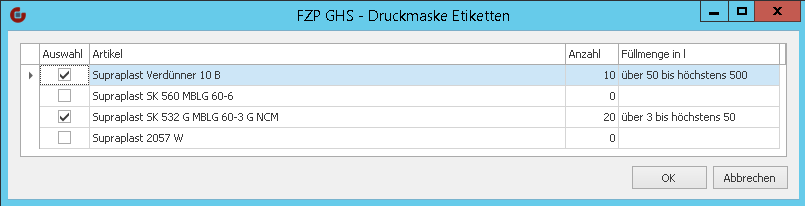
\includegraphics[height=140pt, width=\textwidth]{druckmaske_endprodukt_2.png}
    \caption[Endprodukt der Druckmaske]
    {\small{Endprodukt der Druckmaske}}
    \label{fig:epdruckmaske}
\end{figure}

\noindent
Die zweite Möglichkeit ist der Aufruf der Druckmaske nach dem Speichern eines Verkaufsbeleges. 
Diese zeigt alle Artikel des jeweiligen Verkaufsbeleges an. Hier kann entschieden werden, für 
welche Artikel Etiketten erstellt werden sollen. Zudem kann die Anzahl und die Größe des
Etiketts angegeben werden (siehe Abbildung \ref{fig:epdruckmaske}). Die Größe des Etiketts wird 
anhand der Füllmenge bestimmt, wie im Abschnitt \ref{subsubsec:erstellungetiketten} der Konzeption beschrieben. 
Mit Betätigung der OK Schaltfläche wird die Etikettenerstellung ausgelöst. Das Endprodukt der 
Erstellung ist in Abbildung \ref{fig:epetikett} zu sehen. Die Erstellung der Etiketten wird auszugsweise 
im Listing \ref{code:etiketten} beschrieben.

\begin{figure}[H]
    \centering
    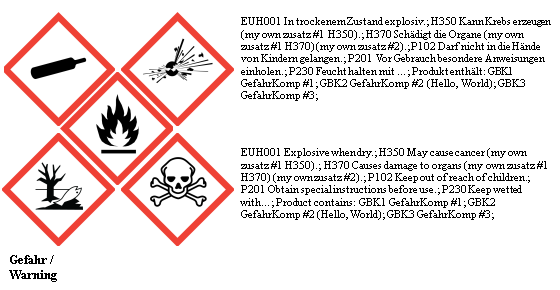
\includegraphics[height=210pt, width=\textwidth]{musteretikett_endprodukt.PNG}
    \caption[Endprodukt der Etiketten]
    {\small{Endprodukt der Etiketten (ohne kundenspezifischer Angaben)}}
    \label{fig:epetikett}
\end{figure}

\begin{lstlisting}[style=A, caption=Auszug Routine Etikettenerstellung (.NET),
label={code:etiketten}]
    Public Class frmGhsAuswahlEtiketten
        ...
        '# Aufruf Methode zur Etikettenerstellung im Formular mittels OK Button
        '# ----------------------------------------------------------------
        '# Die eingegebenen Daten werden aus der GridView in eine DataTable 
        '# uebergeben und eine neue Instanz des Objekts zur Auswahl der Etiketten
        '# mittels der uebergebenen Daten erzeugt. Anschlieszend wird die Methode 
        '# "CreateReportGHSEtiketten()" aufgerufen die die Etiketten erstellt. 
        Private Function SaveFormular() As Boolean
            ...
            Dim druckAuftraege As DataTable = dataRows.CopyToDataTable
            Dim ghsEtikettenAuswahl As New GHSEtikettenAuswahl(druckAuftraege)
            ghsEtikettenAuswahl.CreateReportGHSEtiketten() 
            ...
        End Function
        ...
    End Class
    
    Public Class GHSEtikettenAuswahl
        ...
        '# Die uebergebene DataTable wird zeilenweise durchgegangen und
        '# anhand der Fuellmenge wird entschieden welches Etikettenformat
        '# genommen werden soll. Anschlieszend wird Methode "CreateEtiketten()"
        '# ausgefuehrt die die Etiketten anhand der Anzahl der Piktogramme erstellt.
        Public Function CreateReportGHSEtiketten() As Boolean
            For Each row As DataRow In _dtDruckAuftraege.Rows
                Dim artikelNummer As String = FZPCStr(row.Item("Artikelnummer"))
                Dim artikelZielland As String = FZPCStr(row.Item("Zielland"))
                Dim auswahlEtikettenFormat As Integer = FZPCInt(row.Item("Fuellmenge"))
                Dim anzahlPiktogramme As Integer = _
                GHSMerkmalHelper.GetAnzahlPiktogrammeForArtikelnummer(artikelNummer)
                ...
                Select Case auswahlEtikettenFormat
                    ...
                    Case EtikettenFormat.A5
                        CreateEtiketten(anzahlPiktogramme, artikelNummer, _
                        artikelZielland, artikelBezeichnung, anzahl)
                        Return True
                End Select
            Next
        End Function
    
        '# Erstellung Etiketten anhand der Piktogrammanzahl mittels der Methode
        '# "CreateGHSEtiketten3PA5()" der Klasse "rptEtikettenGhs3PA5".
        Private Sub CreateEtiketten(ByVal anzahlPiktogramme As Integer, _
          ByVal artikelnummer As String, ByVal artikelZielland As String, _
          ByVal artikelBezeichnung As String, ByVal anzahl As Integer)
            Select Case anzahlPiktogramme
                ...
                Case 3
                    Using report3p As New rptEtikettenGhs3PA5(artikelnummer, _
                      artikelZielland, artikelBezeichnung, anzahl)
                        report3p.CreateGHSEtiketten3PA5()
                    End Using
                ...
            End Select
        End Sub
        ...
    End Class

    Public Class rptEtikettenGhs3PA5
        ...
        '# Zuerst werden die GHS Merkmal Daten anhand der uebergebenen
        '# Artikelnummer von der Datenbank geladen. Danach wird die Zweitsprache
        '# fuer das Etikett bestimmt. Anschlieszend werden die Etiketten mittels
        '# der Methode "PrepareEtikett()" erstellt. Im letzten Schritt werden 
        '# die erzeugten Etiketten dem Anwender mit der Anweisung
        '# "mainReport.ShowPreviewDialog()" zum drucken angezeigt.
        Public Sub CreateGHSEtiketten3PA5()
            Dim ghsMerkmale As DataTable = 
            GHSMerkmalHelper.GetGhsMerkmaleForArtikelnummerAsDataTable(_artikelNummer)
            Dim ghsMerkmaleZweitsprache As DataTable
    
            If "DE".Equals(_artikelZielland) Then
                ghsMerkmaleZweitsprache = 
                GHSMerkmalHelper.GetGhsMerkmaleForArtikelnummerAsDataTable( _ 
                _artikelNummer, False, 0, Nothing, "EN")
            Else
                ghsMerkmaleZweitsprache = 
                GHSMerkmalHelper.GetGhsMerkmaleForArtikelnummerAsDataTable( _ 
                _artikelNummer, False, 0, Nothing, _artikelZielland)
            End If
    
            Dim mainReport As New XtraReport
            mainReport.PaperKind = Printing.PaperKind.A4
    
            For i As Integer = 1 To _anzahl
                If Me.PrepareEtikett(ghsMerkmale, ghsMerkmaleZweitsprache) Then
                    Me.CreateDocument()
                    mainReport.Pages.Add(Me.Pages.Item(0))
                End If
            Next
    
            mainReport.ShowPreviewDialog()
        End Sub
        
        '# In dieser Methode werden alle GHS Merkmale mit dem Etikett
        '# verknuepft, z.B. mit den Anweisungen "Me.pbPiktogramm1.Image" 
        '# oder "Me.lblSignalwort.Text".
        Private Function PrepareEtikett(ByVal ghsMerkmale As DataTable, _
          ByVal ghsMerkmaleZweitsprache As DataTable) As Boolean
            If ghsMerkmale Is Nothing Then Return False
            ...
            Dim piktogrammRows As List(Of DataRow) = (From row As DataRow _ 
            In ghsMerkmale.AsEnumerable Where row.Field(Of String) _
            ("MerkmalId").StartsWith("GHS")).ToList
            
            For Each row As DataRow In piktogrammRows
                If piktogrammRows.IndexOf(row) = 0 Then
                    Me.pbPiktogramm1.Image = 
                    ImageHelper.ResizePiktogramm(GetImageFromResource( _
                    FZPCStr(row.Item("MerkmalId"))), 115, 115)
                End If
                ...
            Next
    
            Dim sbSW As New System.Text.StringBuilder
            Dim signalwortRows As List(Of DataRow) = (From row As DataRow In _
            ghsMerkmale.AsEnumerable Where row.Field(Of String) _ 
            ("MerkmalId").StartsWith("SW")).ToList
            
            For Each row As DataRow In signalwortRows
                sbSW.Append(FZPCStr(row.Item("Bezeichnung")))
            Next
    
            sbSW.Append(" / ")
    
            Dim signalwortZSRows As List(Of DataRow) = (From row As DataRow In _
            ghsMerkmaleZweitsprache.AsEnumerable Where row.Field(Of String) _
            ("MerkmalId").StartsWith("SW")).ToList
            
            For Each row As DataRow In signalwortZSRows
                sbSW.Append(FZPCStr(row.Item("Bezeichnung")))
            Next
            Me.lblSignalwort.Text = sbSW.ToString
            ...
            Return True
        End Function
        ...
    End Class
\end{lstlisting}
